\subsubsection{UC8 - Copia del \glossario{prompt} generato}\label{UC8}

\begin{figure}[H]
  \centering
  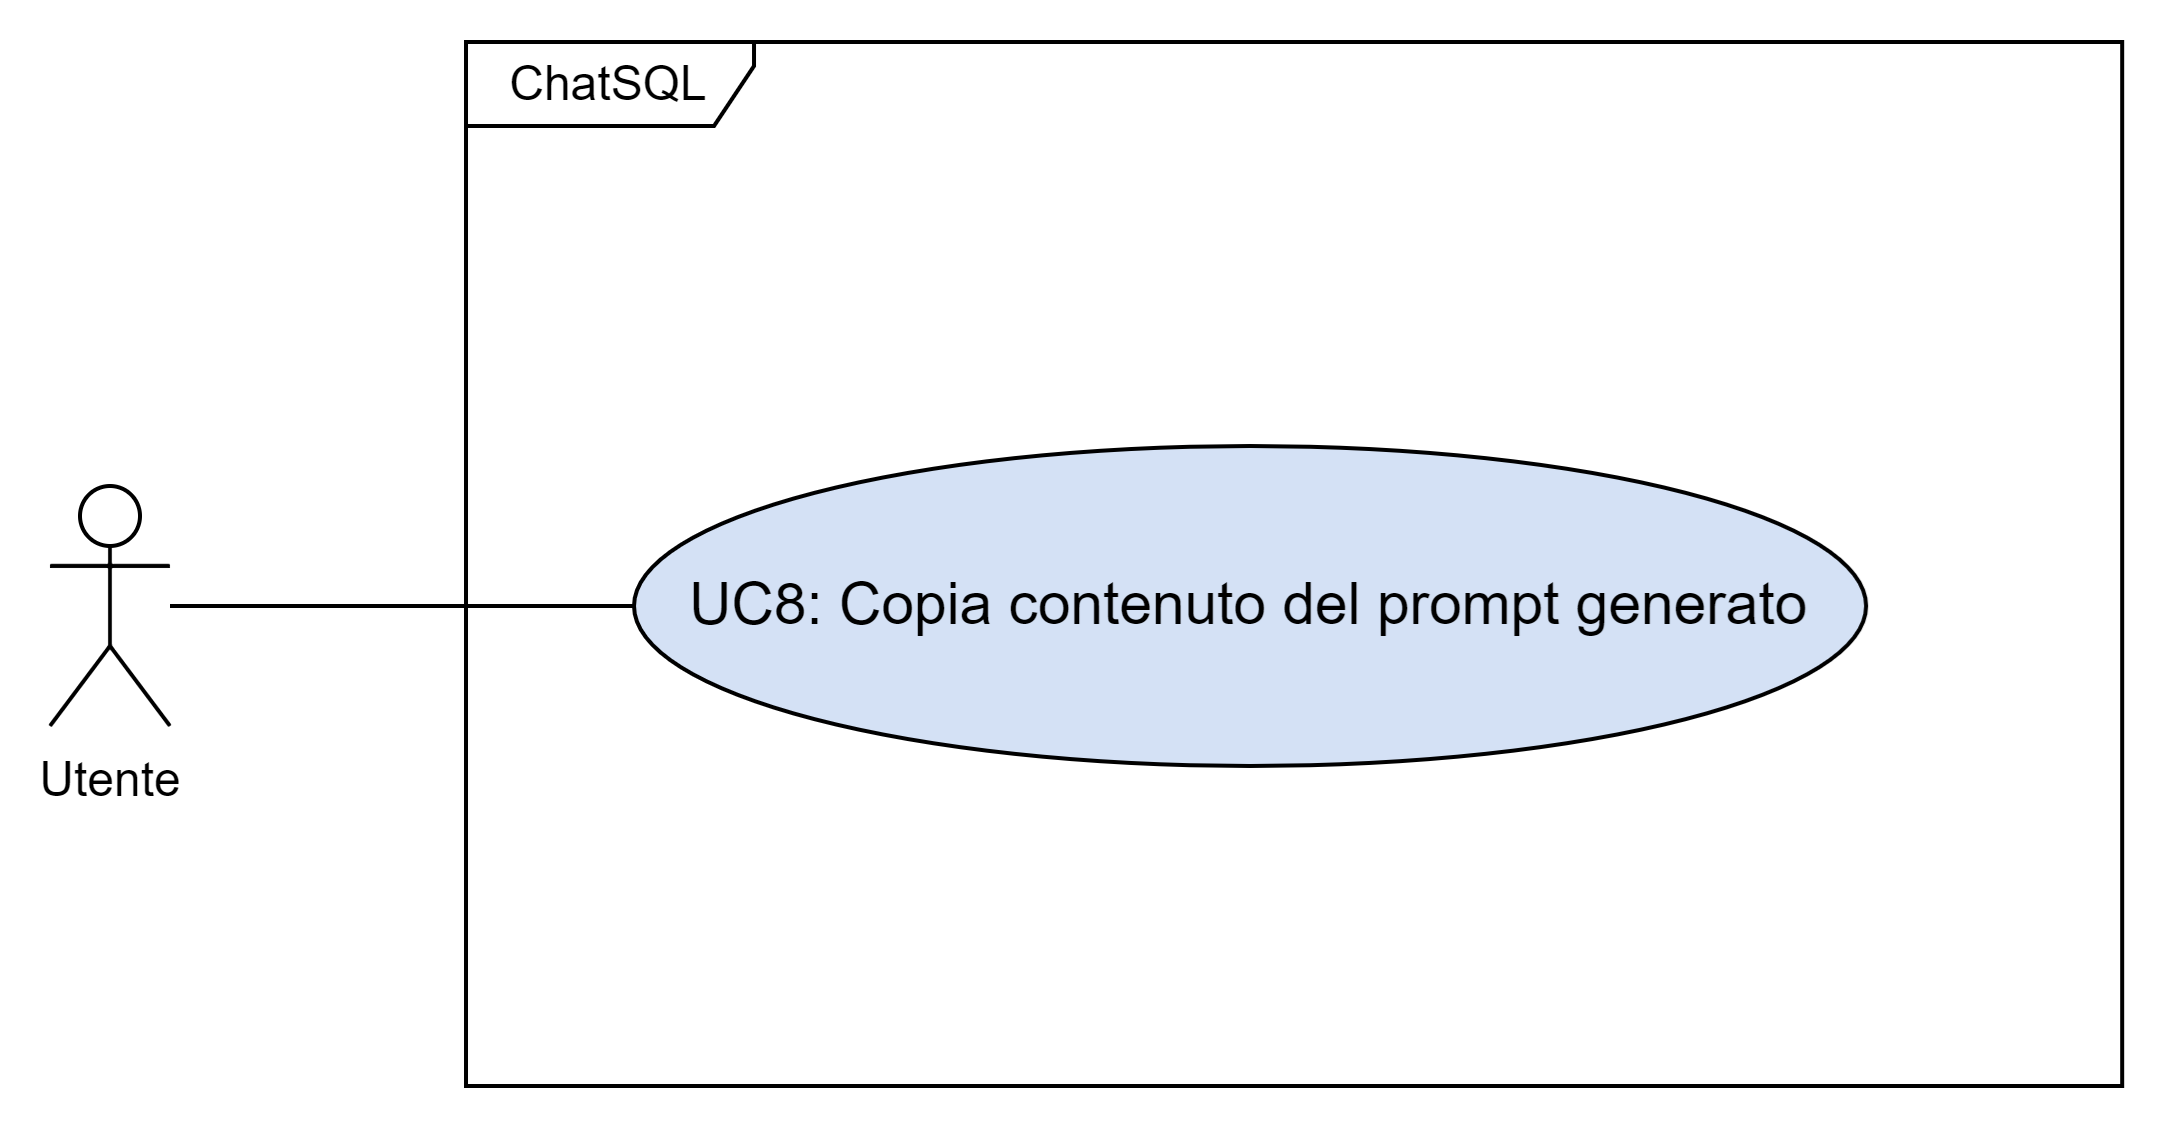
\includegraphics[width=0.90\textwidth]{assets/uc8.png}
  \caption{UC8}
\end{figure}

\paragraph*{Descrizione}
L'Utente può copiare il contenuto del \glossario{prompt} negli appunti di sistema, per poi incollarlo agevolmente in un servizio esterno.

\paragraph*{Attori principali}
Utente

\paragraph*{Precondizioni}
\begin{itemize}
  \item L'applicazione è stata avviata con successo;
  \item Il sistema ha generato almeno un \glossario{prompt}.  
\end{itemize}

\paragraph*{Postcondizioni}
\begin{itemize}
  \item Il \glossario{prompt} viene correttamente copiato negli appunti di sistema dell'Utente.
\end{itemize}

\paragraph*{Trigger}
L'Utente desidera copiare il \glossario{prompt} generato, con l'obiettivo di effettuare un'operazione di "Copy and Paste", incollando il contenuto del prompt in un servizio esterno che implementi \glossario{LLM}.

\paragraph*{Scenario principale}
\begin{enumerate}
  \item L'Utente visualizza il \glossario{prompt} generato;
  \item L'Utente seleziona la funzione di copia;
  \item Negli appunti di sistema viene salvata una copia del \glossario{prompt}, che può essere fornita in input a un \glossario{LLM} esterno per la generazione di una \glossario{query} SQL.
\end{enumerate}